%\renewcommand{\lastmod}{April 27, 2020}


\chapter{Molecular Aggregates --- Coupled Two-Level Systems}
\label{chap:molecular_aggregates}


\section{Tasks}

\begin{itemize}
\item The data contains absorption spectra of the molecule TDBC in solution at different concentrations. Determine the number of chromophores that contribute to the delocalized state. Data by Tobias Kroh, Bayreuth.

\item The second data set contains emission spectra of TDBC in solution at different concentrations. Plot the normalized emission spectrum and discuss. Data by Tobias Kroh, Bayreuth.
\end{itemize}


%\section{Experiment}




\section{Coupled Pendulum}

A mathematical pendulum of point mass $m$ and rod length $L$ is governed by the differential equation of its angular displacement $\phi$
\begin{equation}
 \ddot{\phi} + \frac{g}{L} \, \phi = 0 \quad \text{with} \quad \omega^2 = \frac{g}{l}  \quad , 
\end{equation}
where $g$ is the acceleration due to gravity and $\omega$ its angular eigen-frequency. When two of such pendula are coupled by a spring between the two masses, we get a coupled system of differential equations
\begin{eqnarray}
 \ddot{\phi_1} + \frac{g}{L_1} \, \phi_1  + \frac{k}{m_1} \, \left( \phi_1  - \phi_2 \right)  & = &  0  \\
 \ddot{\phi_2} + \frac{g}{L_2} \, \phi_2  - \frac{k}{m_2} \, \left( \phi_1  - \phi_2 \right)  & = &  0  
\end{eqnarray}
with the spring constant $k$.  For the moment, we assume that the pendula are identical, i.e., $L = L_1 = L_2$ and $m = m_1 =m_2$. The eigen-frequencies are then
\begin{equation}
 \omega_{+}^2 = \frac{g}{L} \quad \text{and} \quad 
  \omega_{-}^2 = \frac{g}{L}  + 2 \frac{k}{m} \quad ,
\end{equation}
where in the mode with frequency $\omega_{+}$ both masses move to the same direction, in the $\omega_{-}$ in opposite directions. Only in the latter case the coupling spring comes into play.

To investigate the general case, we assume harmonic oscillations, i.e. $\phi(t) = \phi_0 \, \exp (i \omega t)$ and write the differential equation as matrix
\begin{equation} \boldsymbol{M \, \phi}	 = 
\begin{pmatrix}
  \frac{g}{L_1} +  \frac{k}{m_1}&  - \frac{k}{m_1}\\
 - \frac{k}{m_2} &  \frac{g}{L_2} +  \frac{k}{m_2}
\end{pmatrix}  \boldsymbol{\phi}	= \omega^2   \, \boldsymbol{\phi}
\quad .
\end{equation}
We thus search eigen-values and eigen-vectors of  $\boldsymbol{M}$. Assuming individual lengths, but identical masses, we get
\begin{equation}
 \omega_{\pm}^2 = \left( \frac{\omega_1^2 + \omega_2^2}{2}  + \frac{k}{m} \right)
  \pm \sqrt{  \left( \frac{\omega_1^2 - \omega_2^2}{2}   \right)^2 + \left(  \frac{k}{m} \right)^2 } \quad .
\end{equation}
For identical lengths, i.e., identical eigen-frequencies $\omega_1 = \omega_2$, this recovers the results from above.


\section{Quantum Mechanics of Coupled States}

A quantum mechanical state is described by its eigen-functions $\psi_i$ and the corresponding eigen-energies $E_i$ so that 
\begin{equation}
\hat{H}  \, \psi_i = E_i  \,\psi_i  \quad .
\end{equation}
The eigen-functions $\psi_j$ form a basis. We can describe all wave functions $\phi$ as
\begin{equation}
\phi = \sum_n \, c_n \, \psi_n \quad.
\end{equation}
In the same way, all operators $\hat{A}$ are fully described by their matrix element
\begin{equation}
 A_{ij} = \braket{ \psi_i | \hat{A} | \psi_j}
\end{equation}
where the brackets describe the integral over all relevant coordinates. We can then\sidenote{For details see a book on quantum mechanics, for example \cite{Schwabl2002_QM1}, chapter 8. } represent the wave function $\phi$ by a vector of the complex entries $c_n$ and the operator by a matrix of the elements $A_{ij}$.

With two states $\psi_a$ and $\psi_b$ we have
\begin{equation}
\hat{H}_0  = \begin{pmatrix}  E_a & 0 \\ 0 & E_b \end{pmatrix} 
	  \quad .
\end{equation}
The Hamilton operator $\hat{H}_0$ is thus described by a $2 \times 2$ matrix. When the two states $a$ and $b$ are coupled, then the energy of one state depends somehow on the other. In the matrix we include a coupling energy $J$ in the off-diagonal elements
\begin{equation}
\hat{H}_{coupled}  = \begin{pmatrix}  E_a & J \\ J & E_b \end{pmatrix} 
\quad . 
\end{equation}
As a consequence, the original eigen-functions $\psi_0$ are no longer eigen-functions of this coupled Hamilton operator. We find new eigen-functions and eigen-values by diagonalizing $\hat{H}_{coupled}$, so that the diagonal elements become
\begin{equation}
 E_\pm = \frac{E_a + E_b}{2} \pm \sqrt{ \left( \frac{E_a - E_b}{2} \right)^2 + J^2 }
\end{equation}
and the new  eigen-functions are\footcite[eq. 8.10]{Parson}
\begin{equation}
 \psi_{\pm} = 
\sqrt{\frac{1 \pm s}{2}} \,  \psi_a \, \,  \pm \, \, \sqrt{\frac{1 \mp s}{2}}  \, \psi_b \quad ,
\end{equation}
with
\begin{equation}
s = \frac{E_a - E_b}{\sqrt{(E_a - E_b)^2 + (2J)^2}} \quad .
\end{equation}
%
%and the new (not normalized) eigen-functions are\sidenote{A more symmetrical equation is given  in \cite[eq. 8.10]{Parson}}
%\begin{equation}
% \psi_{\pm} = \psi_b + \psi_a \left[ \frac{E_a - E_b}{2 J} \pm \sqrt{ \left( \frac{E_a - E_b}{2 J} \right)^2 + 1  } \, \right]
%\end{equation}
We can distinguish two limiting cases. The coupling energy $J$ can be larger than die energy difference between the two states, i.e. $|J| \gg |E_a - E_b| / 2$. Then then new eigen-energies are split up by $\pm J$ around the average of the old eigen-energies $(E_a + E_b) /2$. The eigen-functions in this situation are symmetric and anti-symmetric combinations of the old eigen-function, i.e. $\psi_\pm = \pm \psi_a + \psi_b$. When the coupling energy is small, i.e. $|J| \ll |E_a - E_b| / 2$, then the new eigen-energies and eigen-functions are close to the old.



\begin{figure}
  % \includestandalone[width=10cm]{\currfiledir anticrossing}
   \inputtikz{\currfiledir/anticrossing_v2}

\caption{Eigen-Energies and weights of the eigen-functions as function of the unperturbed energies ($E_b = 1$).}
\end{figure}

A few side remarks and things that are left open for future versions of this text: 
\begin{itemize} \setlength{\itemsep}{0pt}
    \item When the coupling interaction is the electromagnetic wave, then this formalism describes the AC Stark effect, i.e., the shift of atomic transitions in the presence of strong optical fields.
    \item The coupling constant $\beta$ can be complex-valued, i.e., can include a phase lag.
    \item Preparation and temporal evolution of coupled states could be interesting to discuss.
\end{itemize}




\section{Coupling of two transition dipole moments}


We consider two molecules, $a$ and $b$, each with a ground ($0$) and excited ($1$) state. We write the wave function on the form $\ket{ab}$, i.e. $\ket{01}$ is molecule $a$ in ground state, molecule $b$ in excited state. In each molecule, an optical transition dipole moment couples ground and excited state, i.e. $\braket{10| \hat{\mu}_a | 00}$ and $\braket{01| \hat{\mu}_b | 00}$ are different from zero and describe an excitation of the molecule  $a$ and $b$, respectively. Additionally, the two transition dipole moments interact and lead to a resonant coupling of the 
$\ket{01}$ and $\ket{10}$ state\footcite{knoester-book}
\begin{equation}
\hat{H}_{coupling} = J \left(  \ket{10}\bra{01} + \ket{01}\bra{10}   \right) \quad .
\end{equation}
The coupling energy $J$ depends on distance $\boldsymbol{r}_{ab}$ and relative orientation of the transition dipoles $\boldsymbol{\mu}_{a,b}$. It can be seen as the energy of one dipole in the field of another\sidenote{does this need more details? See Parson}
\begin{eqnarray}
 J & = & \frac{\boldsymbol{\mu}_a \cdot  \boldsymbol{\mu}_b }{|\boldsymbol{r}_{ab}|^3} 
  + 3 \frac{ (\boldsymbol{\mu}_a \cdot  \boldsymbol{r}_{ab})  (\boldsymbol{\mu}_b \cdot  \boldsymbol{r}_{ab})
  }{ |\boldsymbol{r}_{ab}|^5 } \\
   & = & \frac{\mu_a \mu_b }{r_{ab}^3} \left( \cos \theta - 3 \cos \alpha \, \cos \beta \right)  = \frac{\mu_a \mu_b }{r_{ab}^3} \, \kappa  
\end{eqnarray}
where the angles are defined in the sketch.

\begin{marginfigure}
%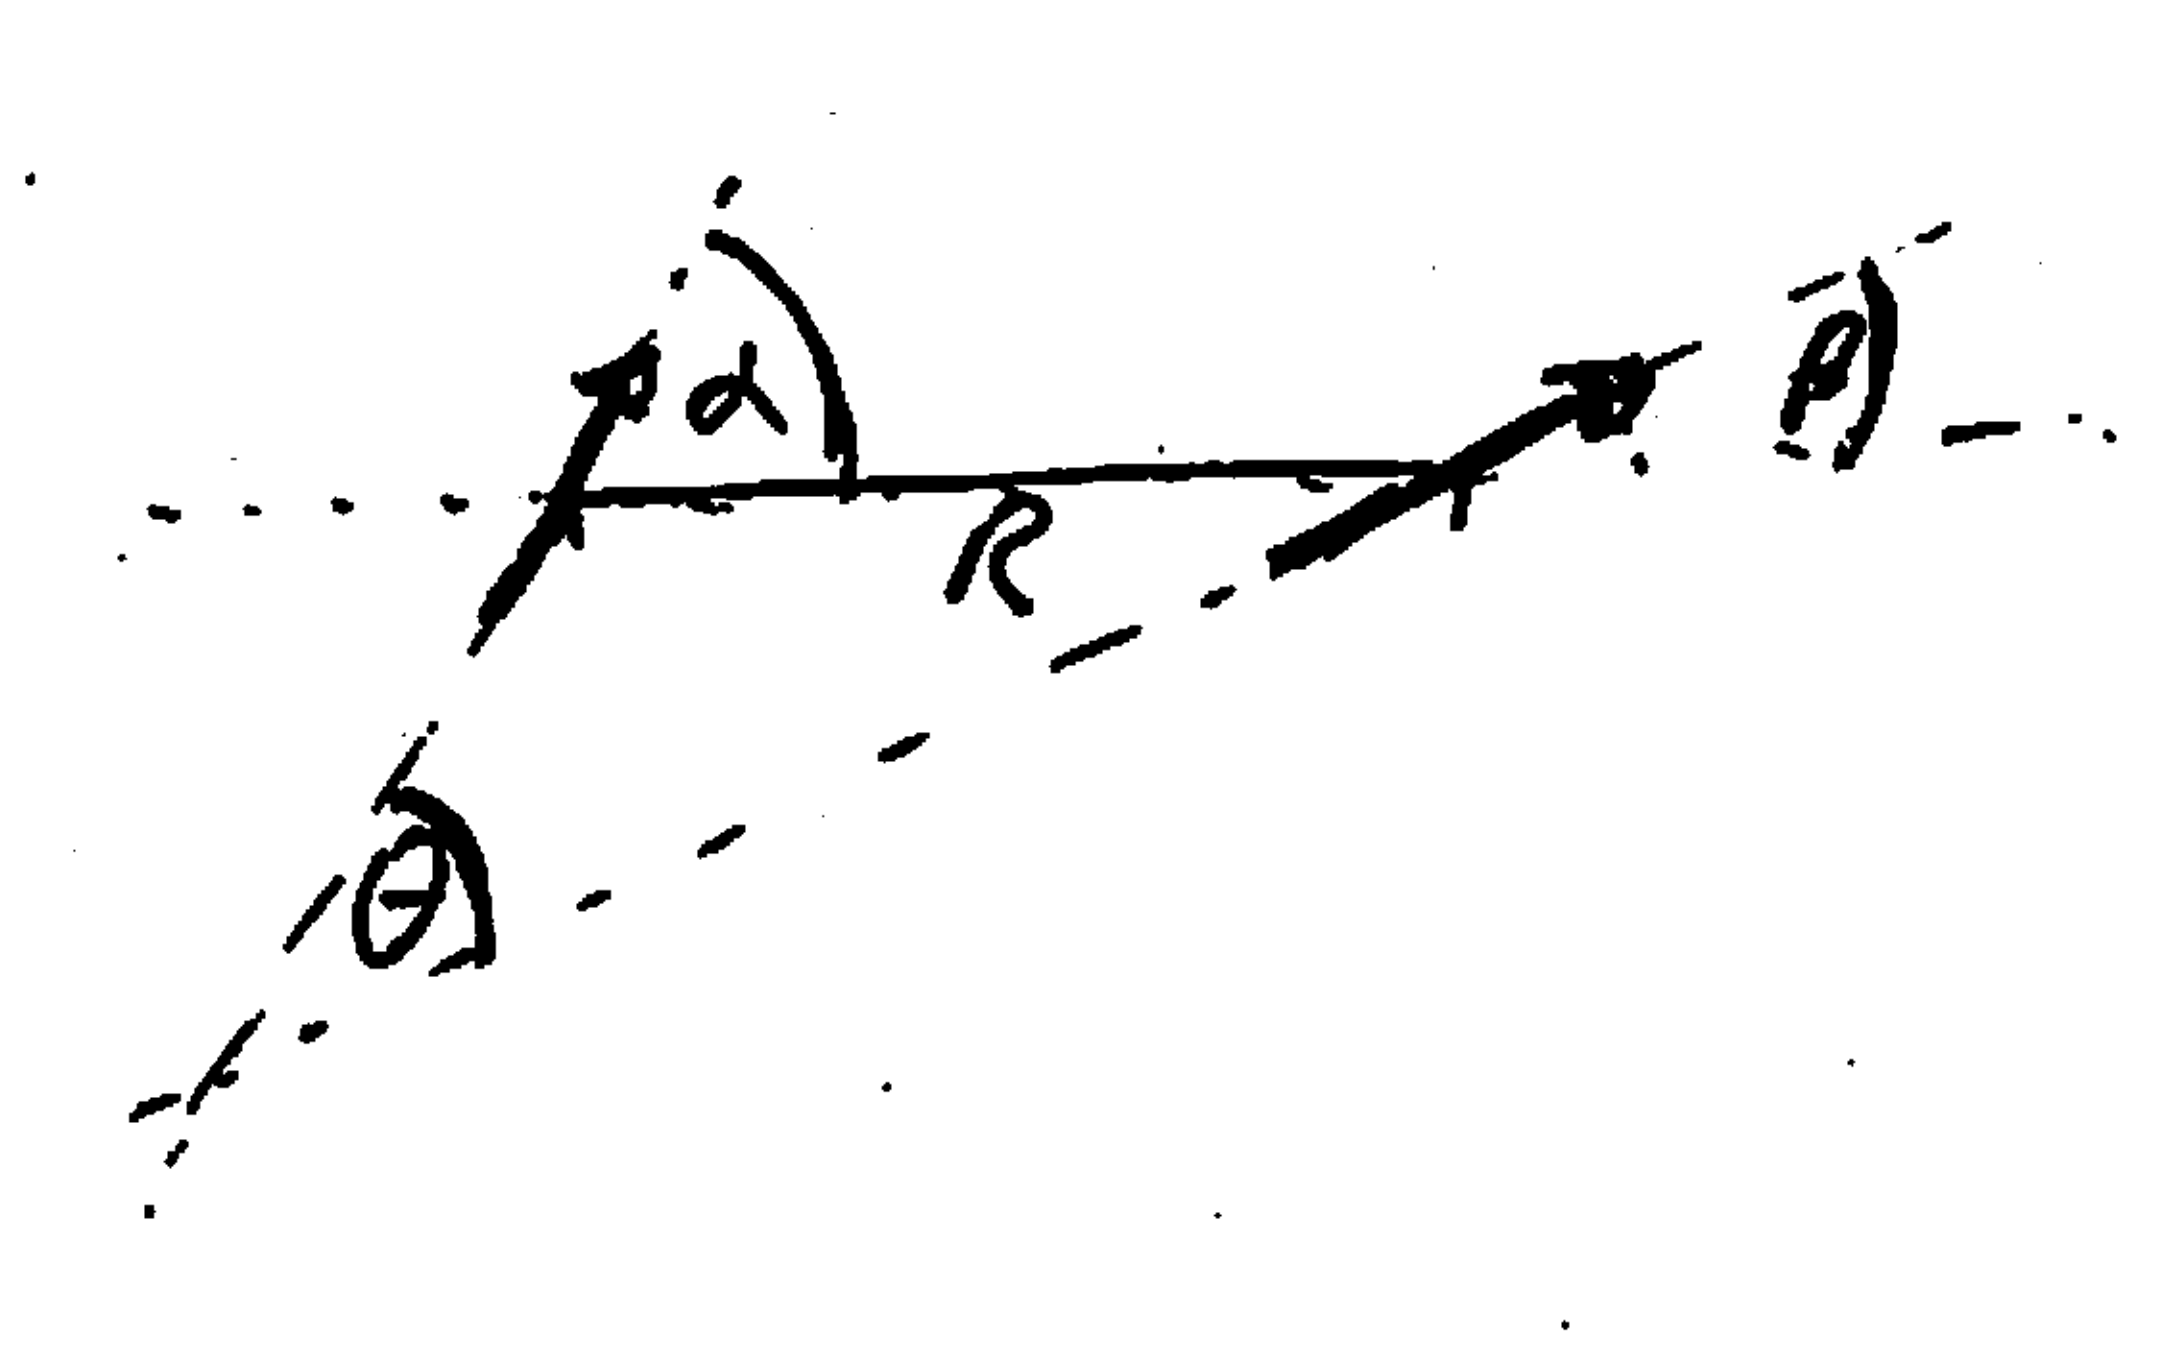
\includegraphics[width=\textwidth]{\currfiledir/angles.png}
   \inputtikz{\currfiledir/angles}

\caption{Sketch showing 
the angles used to calculate the coupling factor $\kappa$}
\end{marginfigure}

A similar coupling term also exist for the non-resonant coupling\footcite{knoester-book}
\begin{equation}
\hat{H}_{non-res} = J \left(  \ket{11}\bra{00} + \ket{00}\bra{11}  \right)
\end{equation}
but this can be ignored, as it is non-resonant. Altogether, the Hamilton operator reads in matrix form
\begin{equation}
\hat{H} = \begin{pmatrix}
0   					& \mu_a 						&	\mu_b						& 		J 		\\
\mu_a^\star	& \hbar \omega_a		&	J								& \mu_b	\\
\mu_b^\star  &  J^\star					& \hbar \omega_b		& \mu_a	\\
J^\star				& \mu_b^\star			& \mu_a^\star			& \hbar (\omega_a + \omega_b) \\
\end{pmatrix} \quad .
\end{equation}
When we ignore the double-excited state $\bra{11}$, the essence in contained in the center $2 \times 2$ matrix which we discussed already in the preceding section.

When $\ket{\psi}$ is a linear combination of $\ket{01}$ and $\ket{10}$, then also the transition dipole moment from $\ket{00}$ to $\ket{\psi}$ is a linear combination of $\mu_a$ and $\mu_b$ with the same weights. When $J \gg |E_a - E_b| / 2$ then we get
\begin{equation}
 \boldsymbol{\mu}_{\pm} = \sqrt{1/2} \, \left( \boldsymbol{\mu}_a \pm  \boldsymbol{\mu}_b  \right)  \quad .
\end{equation}
The brightness of the absorption line is for identical molecules, i.e. $\mu = \mu_a = \mu_b$
\begin{equation}
 I \propto |\boldsymbol{\mu}_{\pm}|^2 = (1/2) \, \left| \boldsymbol{\mu}_a \pm  \boldsymbol{\mu}_b  \right|^2 =  \left( 1 \pm \cos \theta \right) \, \left| \boldsymbol{\mu}   \right| ^2  \quad ,
\end{equation}
where $\theta$ is as above the angle between the transition dipole moments. The same relation hold for the radiative rate.

The spectroscopic signature of coherent coupling between two molecules is thus a splitting of the absorption line into two lines, separated by twice the coupling energy $J$. The sum of the line amplitudes remains unchanged, but in some cases (H- and J-aggregates, see below) one transition will take the whole amplitude and the other remains dark. In these cases, no splitting but a shift of the absorption line is observed. The coupling vanishes when both dipoles are oriented perpendicular to each other ($\theta = 90^\circ$)


\section{H- and J-aggregates}

\begin{marginfigure}
%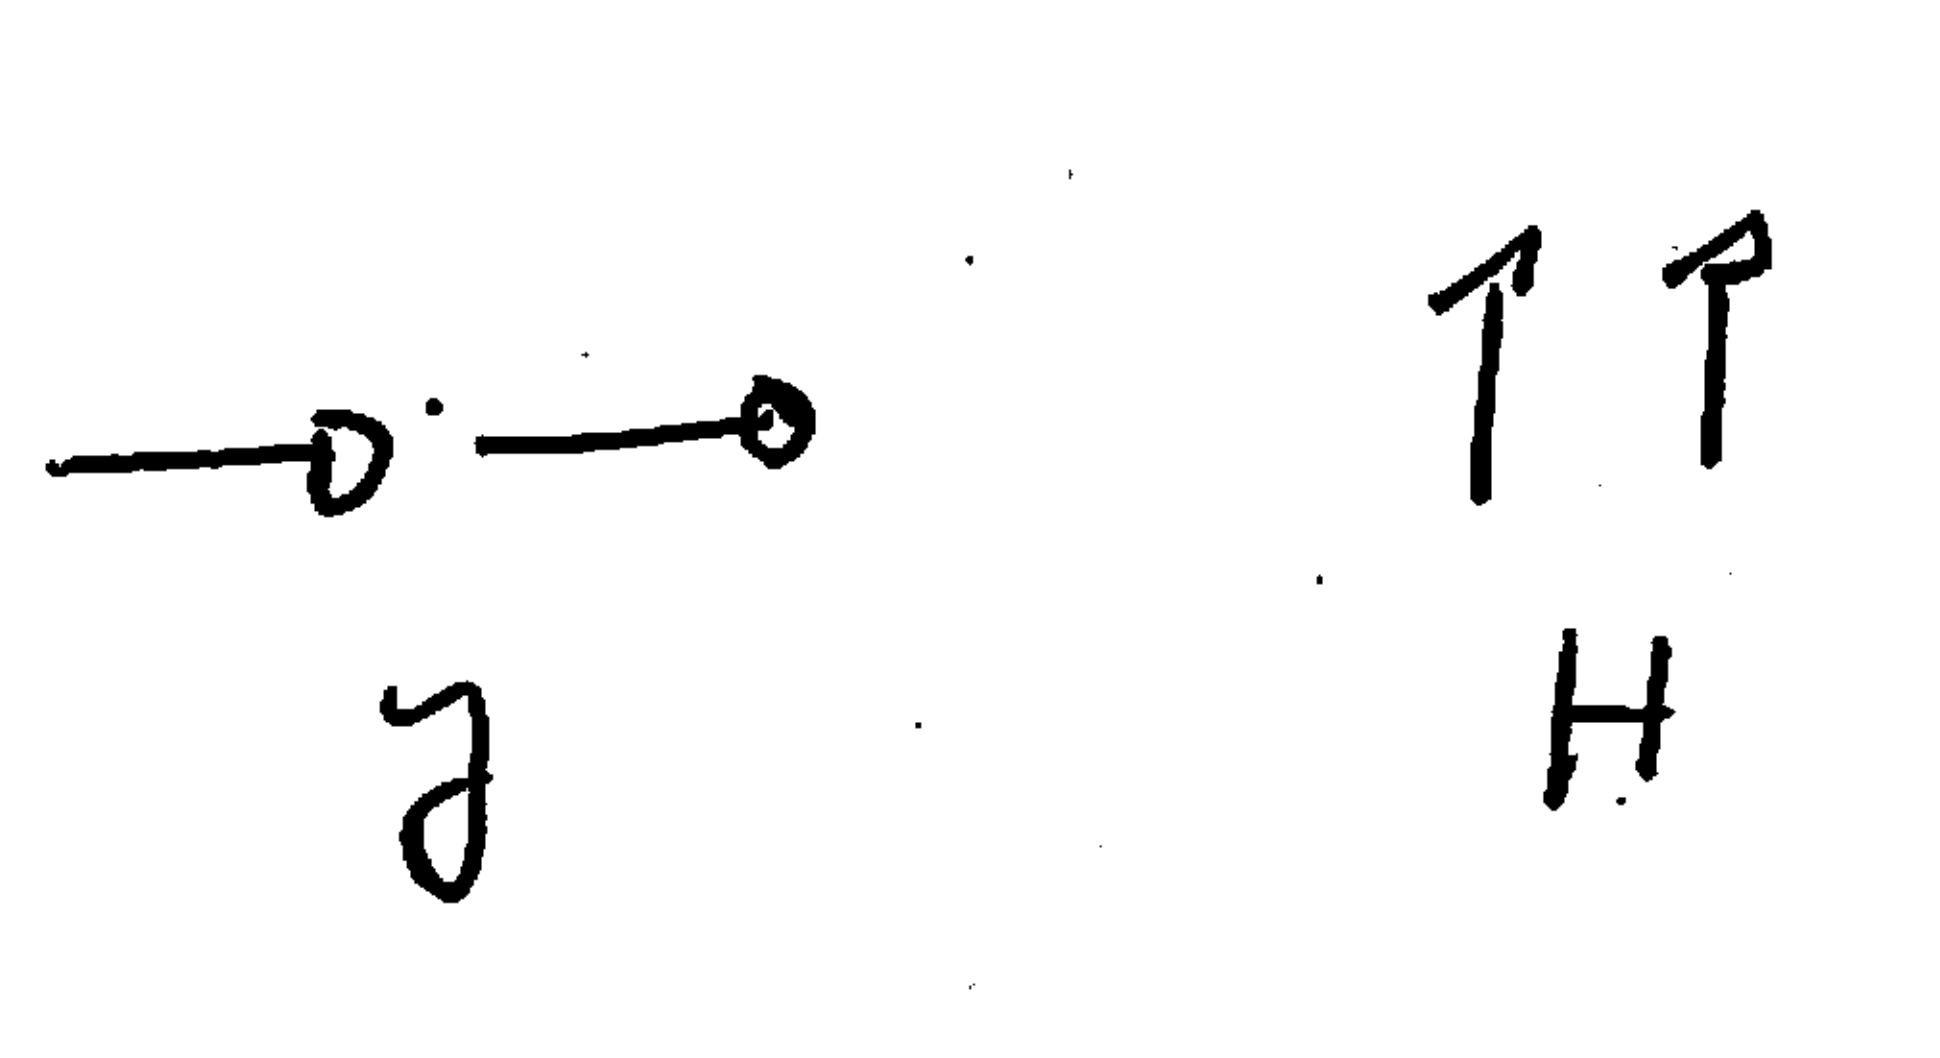
\includegraphics[width=\textwidth]{\currfiledir/aggregates.png}
   \inputtikz{\currfiledir/jh}

\caption{J- and H aggregates.}
\end{marginfigure}


Two important limiting cases are the H- and J-aggregates\footcite[chapters 2.1.4.3, 2.2.5.3]{KoehlerBaessler2015} In a J-aggregate, the dipoles are oriented parallel and head-to-tail, i.e. $\alpha = \beta = \theta = 0$ and therefore $\kappa = -2$. A negative $\kappa$ implies that the coupling constant $J$ is negative. The state $\Psi_+$, which carries all the oscillator strength, has the energy $E_+ = (E_a + E_b) / 2 + J$, which is lower than the average energy of the uncoupled states. The absorption line thus shifts to the red. The same hold for the fluorescence emission spectrum.

In an H-aggregate, the dipoles orient also parallel, but side-to-side, i.e.  $\alpha = \beta = 90^\circ$ and $\theta = 0$. In this case is $\kappa =1$ and $J$ positive. The absorption line shifts to the blue upon formation of aggregates, as again the  $\Psi_+$ state gets all the oscillator strength. However, as fluorescence emission is slow compared to other relaxation processes, this high energy state does not emit light. In emission, H-aggregates appear dark.

The width of the absorption line of a dye at room temperature is determined by dephasing, i.e., fluctuations in the environment that are fast compared to the lifetime of the excited state, and by static differences in the environment of different chromophores. The spectral position of the absorption line in a molecular aggregate is the average of two single chromophore transitions. As in the propagation of uncertainties in an experiment, the width of the new distribution, generated as the average over two values from the old distribution, is reduced by a factor of $\sqrt{2}$. This holds more generally\footcite{Knapp1984}, so that an aggregate of $N$ chromophores is expected to have a spectral line width reduced\sidenote{This is the same physics as motional narrowing in NMR.} by $\sqrt{N}$.




%\begin{tabular}{llll}
%$\theta$	&	$0^\circ$ & $90^\circ$ & $0^\circ$  \\
%$\alpha$ & $0^\circ$ & $0^\circ$ & $90^\circ$  \\
%$\beta$ & $0^\circ$ & $90^\circ$ & $90^\circ$  \\
%$\kappa$  & $-2	$	& 	 $	0	$				& $1$   \\
%\end{tabular}




\printbibliography[segment=\therefsegment,heading=subbibliography]
